\documentclass[serif,mathserif, 12pt]{beamer}
\usepackage{amsmath, amsfonts, epsfig, xspace}
\usepackage{algorithm,algorithmic}
\usepackage{pstricks,pst-node}
\usepackage{multimedia}
\usepackage[normal,tight,center]{subfigure}
\usepackage{siunitx}
\setlength{\subfigcapskip}{-.5em}
\usepackage{beamerthemesplit}
\usetheme{lankton-keynote}

\author{Matthew Willy}

\title[Arduino Demo\hspace{2em}\insertframenumber/\inserttotalframenumber]{Introduction to Arduino}

\date{\today}

\institute{RSI}

\begin{document}

\maketitle

\begin{frame}
  \frametitle{Introduction}
  Topics for today
  \begin{itemize}
  \item Blinking the built in LED (Hello World of Arduino)\pause
  \item Blinking an LED from the breadboard\pause
  \item A simple stoplight demo %leave out the \pause on the final item
  \end{itemize}
\end{frame}

\begin{frame}{Blinking Light Demo}
    The Hello World of Arduino
\end{frame}

\begin{frame}{Two Important Functions}
    
    In every arduino sketch you will have two functions
    
    \begin{itemize}
        \item \textit{setup()}
        \item This is where all of your setup code will go, and runs once, when the arduino is powered on
        or reset. \pause
        \item \textit{loop()}
        \item The main function of your program. An infinite loop that will do all the work.
    \end{itemize}

\end{frame}

\begin{frame}{Simple Breadboard Usage}
    \frametitle{Breadboard}
    \begin{figure}
        \centering
        \subfigure[Breadboard]{
            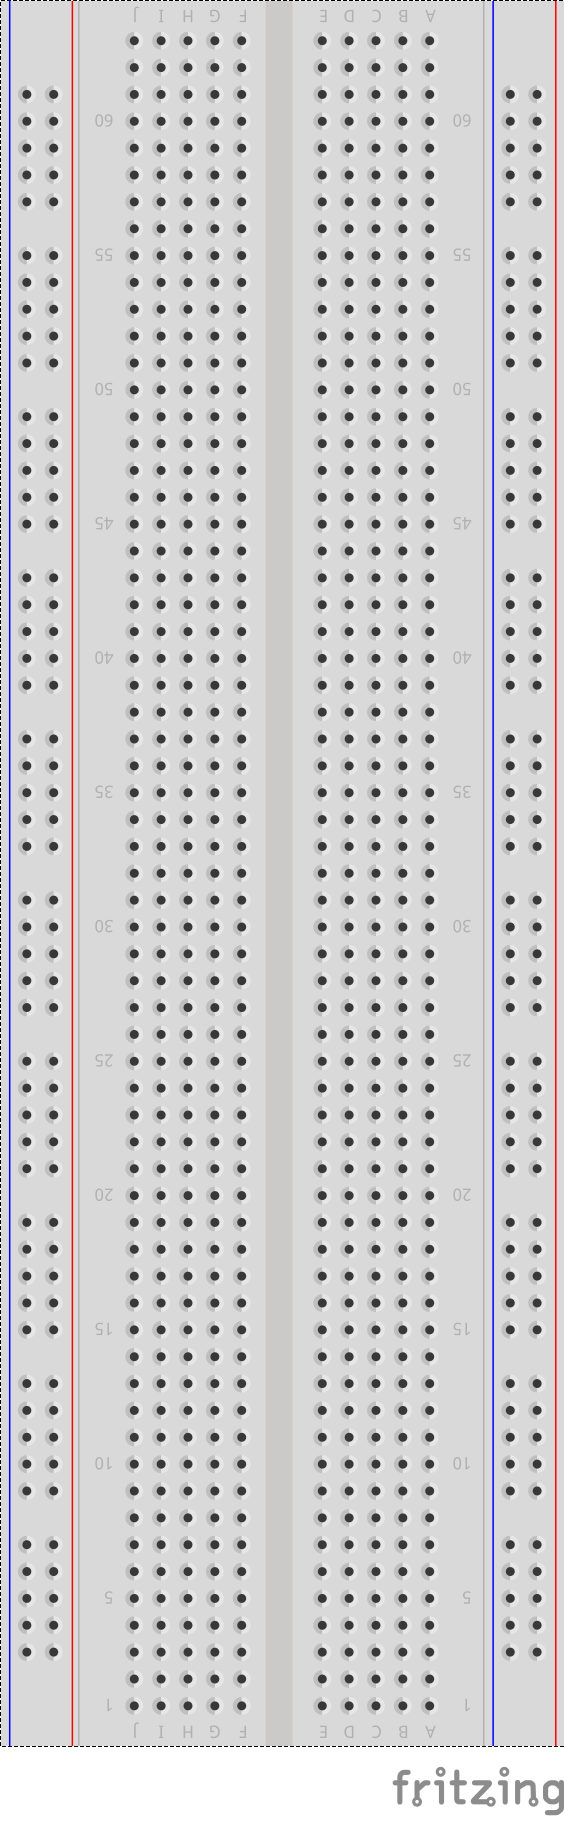
\includegraphics[width=6cm]{images/Breadboard.png}}
        
    \end{figure}
\end{frame}

\begin{frame}{Blinking Light 2.0}

    \begin{figure}
    \centering
    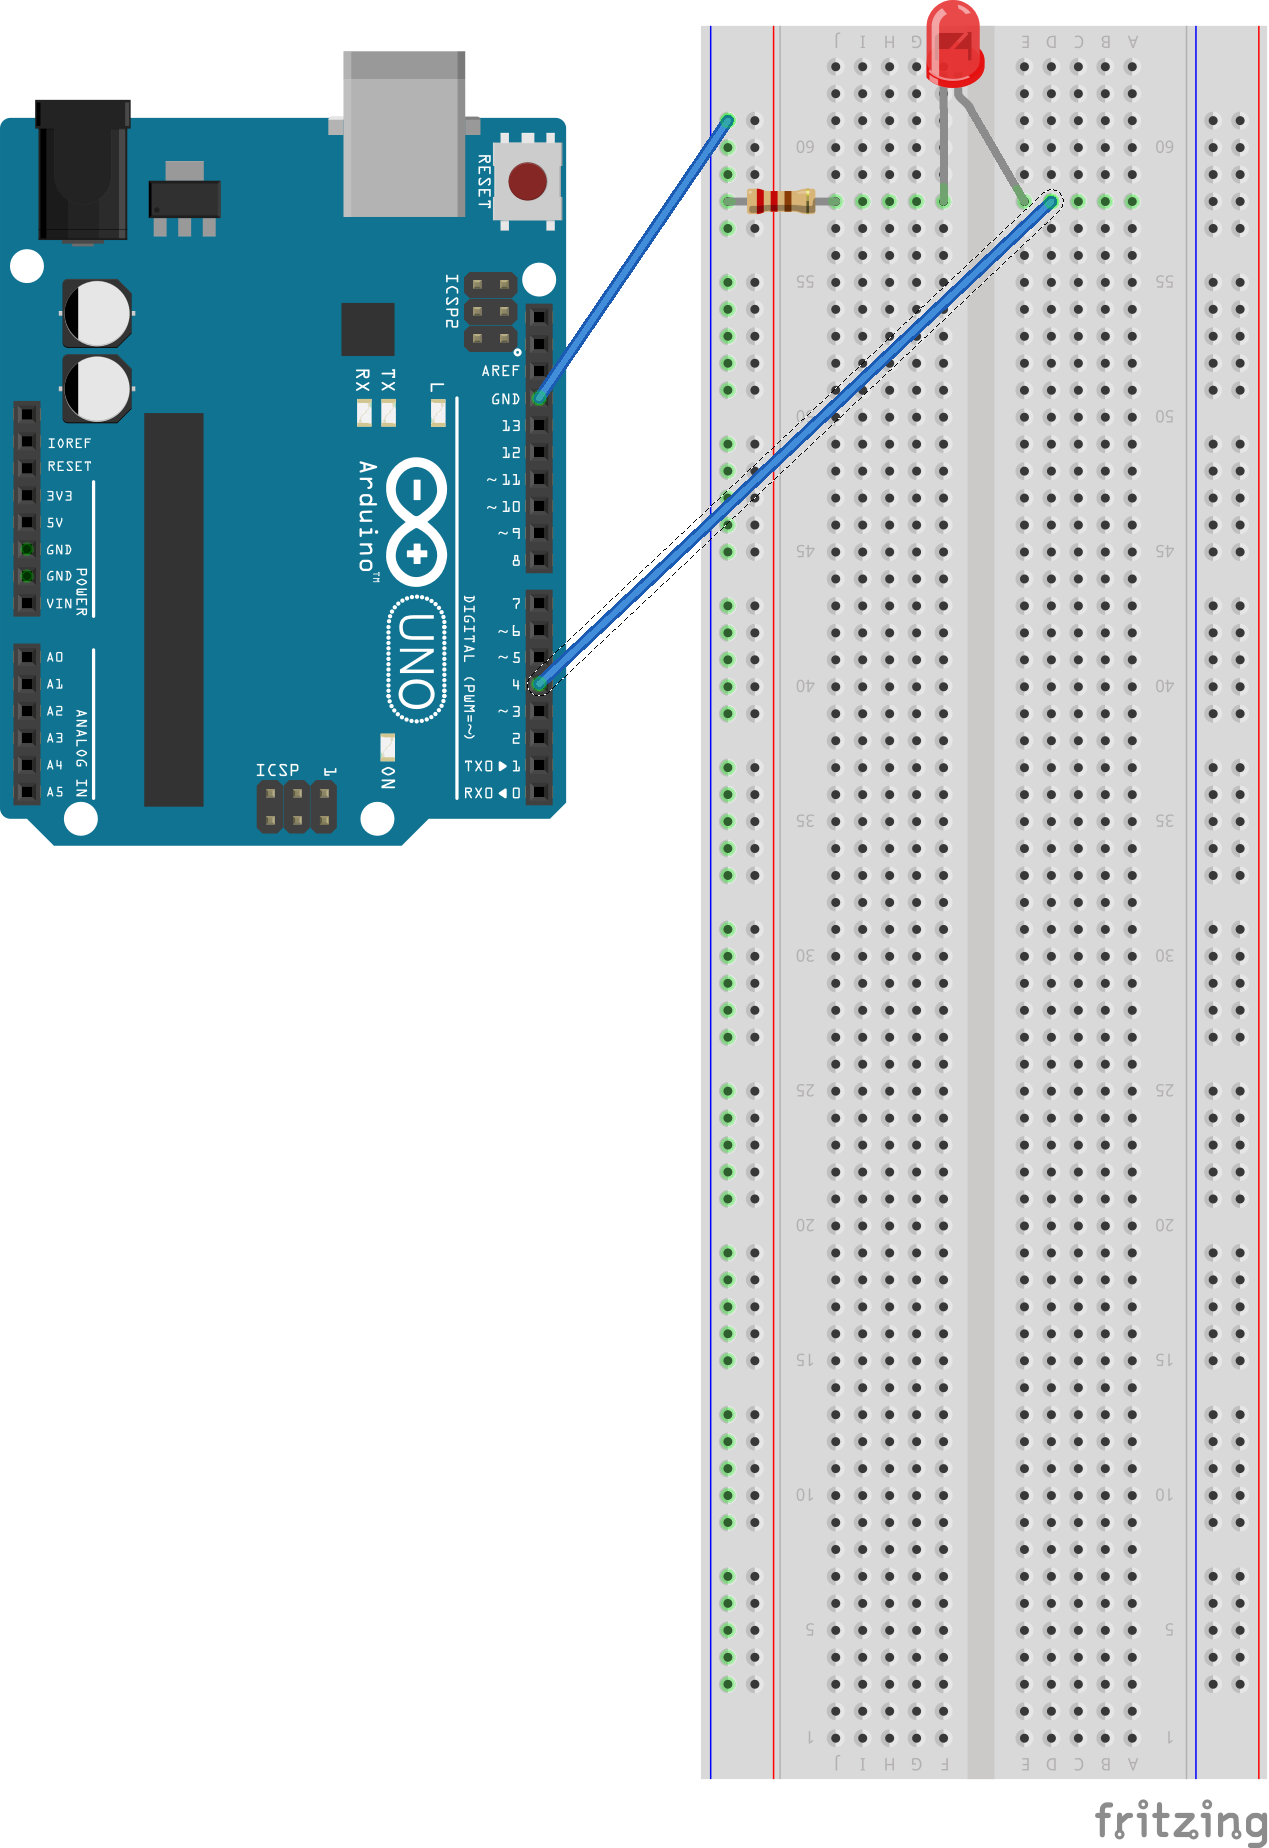
\includegraphics[width=6cm]{images/BlinkingLight.png}
    \end{figure}

\end{frame}

\begin{frame}{It Doesn't Work, Help!}
    \begin{itemize}
        \item Diodes only allow current to pass through in one direction\pause
        \item This means if your LED is plugged in backwards the LED will not light up \pause
        \item \textbf{Quick tip:} The longer of the two leads is the positive end \pause
    \end{itemize}
\end{frame}

\begin{frame}{My LED Burned Out! What??}
    \begin{itemize}
        \item When the LED is plugged directly into the arduino it draws too much current \pause
        \item This will result in burning out the LED, and will release the magic smoke. \pause
        \item How do I stop my LEDs from burning out?? \pause
    \end{itemize}
\end{frame}

\begin {frame}{Resistors to the Rescue!}
    The most basic, and also important equation in electronics
    
    V = I * R \pause
    
    \begin{itemize}
        \item V - Voltage \pause
        \item I - Current \pause
        \item R - Resistance
    \end{itemize}
\end{frame}

\begin{frame}{Calculate Minimum Required Resistance}
    \[R = (V_{\textbf{s}} - V_{\textbf{f})} / I_{\textbf{f}} \] \pause
    \begin{itemize}
        \item R = (5V - 2V) / 0.02A \pause
        \item R = \SI{150}{\ohm}
    \end{itemize}
\end{frame}

\begin{frame}{Only One more Equation, I Promise!}
    \[P = V * I \]
    \[P = I^2 * R\]
    \begin{itemize}
        \item \[P = 0.02^2 A * \SI{150}{\ohm}\] \pause
        \item P = 60mW
    \end{itemize}
\end{frame}

\begin{frame}
  \frametitle{Resistor Color Code}
  \begin{figure}
    \centering
    \subfigure[Resistor Color Code taken from http://www.resistorguide.com/]{
    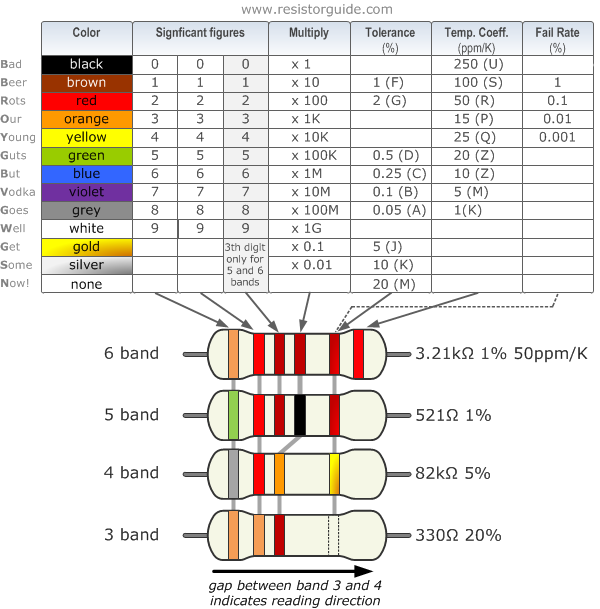
\includegraphics[width=6cm]{images/resistor_color_codes_chart}}
  \end{figure}
\end{frame}

\begin{frame}
    \frametitle{A Word of Caution}
    \begin{alertblock}{Danger}
    Delay is a blocking function. While delay is running you will not
    be able to read sensor inputs, compute mathematical calculations, or
    change pin outputs.
    
    An alternative is to use the \textit{millis()} function instead.
    \end{alertblock}
\end{frame}

\begin{frame}{A Couple of Helpful Resources}
    \begin{itemize}
        \item Fritzing - http://fritzing.org/home/
        \item Arduino - https://www.arduino.cc/
        \item Basic Electronics - https://www.electronics-tutorials.ws/
        \item \LaTeX{} - https://www.sharelatex.com/
    \end{itemize}
\end{frame}

\begin{frame}
  \frametitle{Questions}
  \centering Any Questions?
\end{frame}

\end{document}